%=========================================================================
% sec-opts-attr
%=========================================================================

\section{Experimenting with Attributes}
\label{sec-opts-attr}

% Reason for optimization
\subsection{Reason for Optimization}

Oftentimes the compiler will choose to be conservative with optimization
passes because there is not enough information from static analysis to
determine whether or not certain optimizations are safe. If the
programmer can give hints to the compiler about the intent of the code,
we can force the compiler to make aggressive optimizations to generate
higher performance binaries.
\smallskip

% Details of optimization
\subsection{Details of Optimization}

One significant compiler optimization is the inlining of
functions. Inlined functions are not explicitly called (i.e., no jumping
and linking in assembly), but appear to be embedded into point from which
they are called. This eliminates the overhead of the function call,
which can be especially useful when there are many arguments which need
to be communicated through the stack in memory, instead allowing us to
keep arguments in faster, local registers. Although function inlining is
a common pass in compilers, sometimes we need to force the compiler to do
so by using the {\tt{always\_inline}} attribute. Such C attributes can be
prepended to any function declaration.
\smallskip

Another way to give hints to the compiler is the {\tt{restrict}} keyword
in C. Usually, the compiler tends be conservative about pointer
optimizations if it cannot be sure if pointers alias to the same
locations in memory. However, if we know that certain pointers do not
alias, as in the input matrix pointers A/B/C in DGEMM, we can explicitly
mark such pointers as not aliasing in memory. By doing so, we can help
the compiler perform more aggressive pointer optimizations.
\smallskip

We can also use pragmas to mark loops that should be vectorized (i.e.,
{\tt{\#pragma simd}}), or give hints about when to issue prefetch requests
to saturate the memory bandwidth (i.e., {\tt{\#pragma prefetch A}}).
\smallskip

% Results and analysis
\subsection{Results}

%=========================================================================
% fig-opts-attr-results.tex
%=========================================================================

\begin{figure}[b]

  \centering
  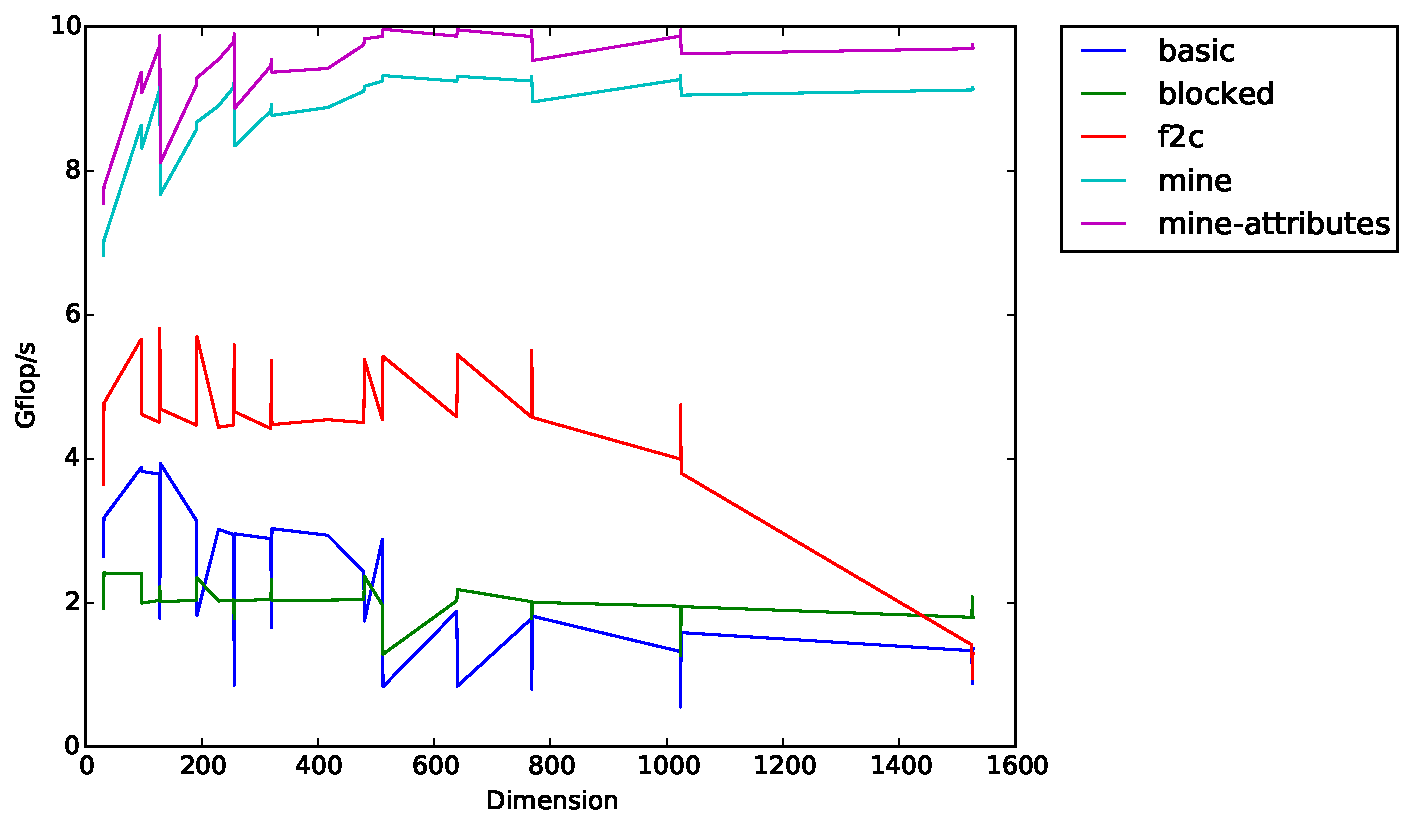
\includegraphics[width=0.7\tw]{fig-opts-attr-results.pdf}

  \caption{\textbf{Performance Comparison of Attribute Optimizations --}
    Results for the blocked implementation with the previous three
    optimizations (i.e., AVX, loop ordering, copy optimization) are shown
    as {\tt{mine}}. Results form adding the compiler hints on top of this
    aggregative implementation are shown as {\tt{mine-attributes}}.  We
    intentionally omit the results for BLAS nad MKL implementations in
    order to focus on the behavior at the performance range of the
    optimization.}

  \label{fig-opts-attr-results}

\end{figure}


Figure~\ref{fig-opts-attr-results} compares the performance of the blocked
DGEMM implementation with the three previous optimizations: AVX, loop
ordering, copy optimization, with and without the additional compiler
hints described above.
\medskip
